% !TeX root = report_example.tex
\newcommand*{\MyHeaderPath}{.}% This path definition is also passed to inside the header files.
\newcommand*{\PathToAssets}{../assets}%
\newcommand*{\PathToOutput}{../output/}%
\newcommand*{\PathToOutputTables}{../output/tables}%
% \newcommand*{\PathToBibFile}{bibliography.bib}%


%%%%%%%%%%%%%%%%%%%%%%%%%%%%%%%%%%%%%%
%% This file is compiled with XeLaTex.
%%%%%%%%%%%%%%%%%%%%%%%%%%%%%%%%%%%%%%

\documentclass[12pt]{article}
%\documentclass[reqno]{amsart}
%\documentclass[titlepage]{amsart}

%% {{{{
%% This package is already loaded by beamer
% https://tex.stackexchange.com/questions/314344/beamer-presentation-compile-error
\usepackage{graphicx}
%% }}}}

%http://tex.stackexchange.com/questions/36797/how-can-i-make-todonotes-use-all-of-the-margin
\usepackage{fullpage}
%\usepackage{showframe}
% \usepackage[paperwidth=210mm,
%             paperheight=297mm,
%             left=50pt,
%             top=50pt,
%             textwidth=345pt,
%             marginparsep=25pt,
%             marginparwidth=150pt,
%             textheight=692pt,
%             footskip=50pt]
%            {geometry}

%% {{{{
% https://tex.stackexchange.com/questions/9796/how-to-add-todo-notes
\usepackage{xargs} % Use more than one optional parameter in a new commands 
\usepackage[dvipsnames]{xcolor}
% \newcommandx{\todoproposal}[2][1=]{\todo[linecolor=Plum,backgroundcolor=Plum!25,bordercolor=Plum,#1]{#2}}
\newcommandx{\todoproposal}[2][1=]{\todo[disable, linecolor=Plum,backgroundcolor=Plum!25,bordercolor=Plum,#1]{#2}}
% \newcommandx{\tododraft}[2][1=]{\todo[#1]{#2}}
\newcommandx{\tododraft}[2][1=]{\todo[disable, #1]{#2}}
% \newcommandx{\thiswillnotshow}[2][1=]{\todo[disable,#1]{#2}}
%% Math environment in todo note
%
% https://tex.stackexchange.com/questions/298404/todonotes-and-reserveda-nested-itemize-enumerate-environments/298405#298405
\newcommand\todoin[2][]{\todo[inline, caption={2do}, #1]{
\begin{minipage}{\textwidth-4pt}#2\end{minipage}}}
% \newcommand\todoin[2][]{\todo[disable, inline, caption={2do}, #1]{
% \begin{minipage}{\textwidth-4pt}#2\end{minipage}}}
%% }}}}


%% {{{{
%http://tex.stackexchange.com/questions/44858/adding-the-word-appendix-to-table-of-contents-in-latex
\usepackage[titletoc, page]{appendix}
%% }}}}

%% {{{{
	
%I'm using this package to put todo notes into my document. Then, I can
%use it to put a list of the todo notes at the end of the document.
\usepackage[textsize=footnotesize]{todonotes}
% \usepackage[disable=true, colorinlistoftodos,prependcaption,textsize=footnotesize]{todonotes}
%This package has some conficts with amsart. To resolve this, I use
%the following code.
\makeatletter
\providecommand\@dotsep{5}
\def\listtodoname{List of Todos}
\def\listoftodos{\@starttoc{tdo}\listtodoname}
\makeatother
%I got this workaround code from the package's documentation:
%http://get-software.net/macros/latex/contrib/todonotes/todonotes.pdf

% %\newcounter{chapter}
% %\numberwithin{section}{chapter}
% \theoremstyle{mydefinition}
% \newtheorem{exercise}{Exercise}
% \newcommand{\newproblem}[2]{\setcounter{exercise}{#1}\addtocounter{exercise}{
% -1}\begin{exercise}#2\end{exercise}}
% \newcommand{\setcontext}[2]{\setcounter{chapter}{#1}\setcounter{section}{#2}}

% \newtheorem*{remark}{Remark}

%% }}}}


%% {{{{
% Bibliography as numbered section
% https://tex.stackexchange.com/questions/88890/how-to-get-the-references-section-to-be-numbered-as-if-it-were-created-via-sect
\usepackage[numbib]{tocbibind}
%% }}}}


%%%%%%%%%%%%5
%%%% >>>>

%%%%%%%%%%%%5


%%%%%%%%%%%%%%%%%%%%%%%%
%% Section Styling
%%%%%%%%%%%%%%%%%%%%%%%%%

 \usepackage{titlesec}

% %\titleformat*{\subsection}{\newpage \Large \bfseries}
% \titleformat*{\subsubsection}{\large\itshape}

% \usepackage[explicit]{titlesec}

% %Start section with new page
% %http://tex.stackexchange.com/questions/9497/start-new-page-with-each-section
% \newcommand{\sectionbreak}{\clearpage}

% %Underlining ruler for subsections
% %http://tex.stackexchange.com/questions/84061/how-can-i-make-a-bold-horizontal-rule-under-each-section-title
% \titleformat{\section}
%   {\normalfont\LARGE\bfseries}
%   {
%   \thesection
%   }
%   {1em}
%   {#1}
%   [{\titlerule[0.8pt]}]

% \titleformat{\subsection}
%   {\normalfont\Large\bfseries}
%   {\thesubsection}
%   {1em}
%   {#1}

% \titleformat{\subsubsection}
%   {\normalfont\normalsize\itshape}
%   {\thesubsubsection}
%   {1em}
%   {#1}


% Change format of \paragraph{...}
% http://tex.stackexchange.com/questions/3881/formatting-a-paragraph-to-look-like-a-section
% \titleformat{\paragraph}[hang]{\normalfont\normalsize\itshape}{\theparagraph}{1em}{}
% \titlespacing*{\paragraph}{0pt}{3.25ex plus 1ex minus .2ex}{1em}


%%%%%%%%%%%%%%%%%%%%%%%%%%%%%%%%%%%%%%%%%%%%%%
%% Change section styling for HW documents %%
%%%%%%%%%%%%%%%%%%%%%%%%%%%%%%%%%%%%%%%%%%%%%%

%%%
% This first method uses the base LaTeX package:
% http://tex.stackexchange.com/questions/85011/section-and-subsection-heading-style

%\def\@seccntformat#1{\csname the#1\endcsname\quad} %default

%\def\@seccntformat#1{Problem \csname the#1\endcsname\quad} 

% %%% 
% % This next one uses the `titlesec` packages. The references I used are
% % here:
% % http://tex.stackexchange.com/questions/140447/changing-section-heading-style
% % http://tex.stackexchange.com/questions/37189/number-subsections-and-subsubsections-but-not-sections
% \usepackage{bookmark}
% \usepackage{titlesec}
% \titleformat{\section}
%   {\normalfont\bfseries\Large}{Problem \thesection}{1em}{}
% \titleformat{\subsection}
%   {\normalfont\large\itshape}{\thesubsection}{1em}{}
% \titleformat{\subsubsection}
%   {\normalfont\normalsize\itshape}{\thesubsubsection}{1em}{}

% % Add proper labels to PDF bookmarks.
% % http://tex.stackexchange.com/questions/156530/how-to-change-the-pdfbookmark-titles-hyperref
% \makeatletter
% \bookmarksetup{%
%   addtohook={%
%     \ifnum\toclevel@section=\bookmarkget{level}\relax
%       \renewcommand*{\numberline}[1]{Problem #1 }%
%     \fi
%   },
% }



%Option to number subsection with letters
% http://tex.stackexchange.com/questions/74529/sections-indexed-with-numbers-subsections-with-letters
% \renewcommand{\thesection}{\Alph{section}}
% \renewcommand{\thesubsubsection}{\thesubsection.\alph{subsubsection}}
% %%%%%%%%%%%%%%%%%%%%%%%%%%%%%%%%%%%%%%%%%%%%%

%% {{{{
%Links, esp. from table of contents
% http://timmurphy.org/2014/03/11/latex-table-of-contents-with-clickable-links/
\usepackage{hyperref}
\hypersetup{
    colorlinks=true, % make the links colored
    linkcolor=blue, % color TOC links in blue
    urlcolor=red, % color URLs in red
    linktoc=all, % 'all' will create links for everything in the TOC
    %citecolor=gray
    citecolor=blue
    }
%% }}}}

\usepackage{setspace}
%% Deal with warnings

% -- Temporarily filter warning. "remreset package is obsolete". This package is likely innocuous.
% https://tex.stackexchange.com/questions/438543/what-to-do-when-an-actively-maintained-package-requires-an-obsolete-package
\RequirePackage{silence}
\WarningFilter{remreset}{The remreset package}

% -- Todo notes margin warning:
\setlength {\marginparwidth }{2cm}

%https://tex.stackexchange.com/questions/3473/blackboard-bold-variants-for-greek-letters
\usepackage[bbgreekl]{mathbbol}

\usepackage{amsmath, amsfonts, amscd, amssymb, amsthm}
\usepackage{url}
\usepackage{enumerate}
\usepackage{float}
\usepackage{bbm}
\usepackage{color,soul}
\usepackage{thmtools}
\usepackage{threeparttable}

%% {{{{

%% When Caption is too wide:
% https://tex.stackexchange.com/questions/110393/too-wide-figure-caption/110453
% \captionsetup{width=0.8\textwidth}

% \usepackage[skip=4pt,font=footnotesize, width=\textwidth]{caption}
\usepackage[font=small]{caption}
% \usepackage{caption}
\usepackage{subcaption}
%% }}}}

%% {{{{
%% Bibliography
\usepackage[round,sort,comma,authoryear]{natbib}
% Include in main .tex file: \newcommand*{\MyHeaderPath}{..path_to_header_files..}%
% \bibliographystyle{rusnat}
% \bibliographystyle{plainnat}   % this means that the order of references
%% }}}}


\usepackage[export]{adjustbox}

%% Biblatex
% \usepackage[natbib=true]{biblatex}
% \addbibresource{../../My_Collection.bib}


\usepackage{mathtools}


%% {{{{
% Scalable font and better handling of accents, etc.
% https://tex.stackexchange.com/questions/664/why-should-i-use-usepackaget1fontenc
% https://tex.stackexchange.com/a/10708/41208
% \usepackage[T1]{fontenc}
\usepackage{lmodern}
%% }}}}

%% {{{
% Doesn't work with beamer
% https://tex.stackexchange.com/questions/314344/beamer-presentation-compile-error#comment766741_314344
% Anyway, loading the packages in different order solves the issue: load bm last. I suggest the order inputenc, fontenc, babel if needed, lmodern, mathtools and finally bm
\usepackage{bm}
%% }}}



\usepackage{dcolumn}

%% Force LaTeX image to appear in the section in which it's declared [duplicate]
% https://tex.stackexchange.com/questions/32598/force-latex-image-to-appear-in-the-section-in-which-its-declared
\usepackage[section]{placeins}

%% Used for making landscape (sidewaystable) tables
%
% From here: https://latex.org/forum/viewtopic.php?t=1493
% Creates sideways table environment 
\usepackage{rotating}


%% For use in making tables with multiple panels
%
% See here: https://tex.stackexchange.com/questions/27971/tables-with-multiple-panels-in-latex-r-and-sweave
\usepackage{tabularx}% http://ctan.org/pkg/tabularx
\newcolumntype{Y}{>{\raggedleft\arraybackslash}X}% raggedleft column X

%% For use in raggedright text justification in regular tabular tables
%
% See here: https://tex.stackexchange.com/questions/12703/how-to-create-fixed-width-table-columns-with-text-raggedright-centered-raggedlef
\usepackage{array}
\newcolumntype{L}[1]{>{\raggedright\let\newline\\\arraybackslash\hspace{0pt}}m{#1}}
\newcolumntype{C}[1]{>{\centering\let\newline\\\arraybackslash\hspace{0pt}}m{#1}}
\newcolumntype{R}[1]{>{\raggedleft\let\newline\\\arraybackslash\hspace{0pt}}m{#1}}

% How to add a forced line break inside a table cell
% https://tex.stackexchange.com/questions/2441/how-to-add-a-forced-line-break-inside-a-table-cell
\usepackage{pbox}


%% For use in making landscape tables
% https://tex.stackexchange.com/questions/3930/how-to-rotate-landscape-table-page-in-pdf
% An interesting alternative that also works is https://tex.stackexchange.com/questions/37220/how-to-adjust-or-remove-page-numbers-on-a-landscape-page-within-a-portrait-docum
\usepackage{geometry}
\usepackage{pdflscape}


\usepackage{bibentry}
\makeatletter
%http://tex.stackexchange.com/questions/141446/problem-of-duplicate-identifier-when-using-bibentry-and-hyperref
\renewcommand\bibentry[1]{\nocite{#1}{\frenchspacing
\@nameuse{BR@r@#1\@extra@b@citeb}}}
\makeatother


% %%%% <<<<

% %% Professional Looking Code listings
% %% http://stackoverflow.com/questions/741985/latex-source-code-listing-like-in-professional-books

% %\usepackage{color}
% \usepackage{xcolor}
% \usepackage{listings}

% %\usepackage{caption}
% \DeclareCaptionFont{white}{\color{white}}
% \DeclareCaptionFormat{listing}{\colorbox{gray}{\parbox{\textwidth}{#1#2#3}}}
% \captionsetup[lstlisting]{format=listing,labelfont=white,textfont=white}

% %% Alternative Font for Code Listings
% %% http://tex.stackexchange.com/questions/33685/set-the-font-family-for-lstlisting
% \usepackage{courier}

% \lstset{basicstyle=\footnotesize\ttfamily,breaklines=true}
% \lstset{framextopmargin=50pt,frame=bottomline}

% %% Line Numbers
% \lstset
% { %Formatting for code in appendix
%     %language=Matlab,
%     numbers=left,
%     stepnumber=1,
%     showstringspaces=false,
%     tabsize=1,
%     breaklines=true,
%     breakatwhitespace=false,
% }

% %% Line Numbers starting form an arbitrary number
% %% http://tex.stackexchange.com/questions/61030/how-can-i-start-the-line-numbering-of-my-listing-by-an-arbitrary-number

% % \begin{lstlisting}[firstnumber=100]
% % for i:=maxint to 0 do
% % begin
% % { do nothing }
% % end;
% % \end{lstlisting}

% %%%% >>>>

%%%% <<<<

%% Examples of using underset and underbrace

% $$
% \frac{\dd \pi^2}{\dd K_1} = 
%   \underbrace{\pd{\pi^2}{K_1} }_\text{direct effect}
%   + 
%   \underbrace{\pd{\pi^2}{x_1^*} \pd{x_1^*}{K_1}}_\text{strategic effect}
%   + \underset{\text{due to the envelope theorem}}
%   {\cancel{ \pd{\pi^2}{x_2^*}\pd{x_2^*}{K_1}}}
% $$
%%%% >>>>


%% Aligning numbers by decimal points in table columns
%https://tex.stackexchange.com/questions/2746/aligning-numbers-by-decimal-points-in-table-columns
\usepackage{siunitx}
% From here:https://ctan.org/pkg/siunitx
% Don't intepret comma as decimal marker
\sisetup{
input-decimal-markers = .
}



%%%% <<<<
%% Packages for tables
\usepackage{booktabs}
\usepackage{multirow}
%\usepackage[table,xcdraw]{xcolor}
%I got the following one from here: http://stackoverflow.com/questions/790932/how-to-wrap-text-in-latex-tables
\usepackage{tabulary}
%% Example Table
% \begin{figure}[h!]
% \centering
% \begin{tabulary}{\linewidth}{C|C|C}
% \toprule
% Actions & Inflow at time $t$ & Inflow at time $t + \dd t$     \\ \midrule
% Buy and sell call & $-C$ & $C + \dd C$ \\ \hline
% Short $\alpha$ shares & $\alpha S$ & $-\alpha (S + \dd S)$ \\ \hline
% Buy and sell $\beta$ of option $\hat C$ & $-\beta \hat C$ & $\beta (\hat C + \dd \hat C)$ \\ \hline
% Borrow & $C - \alpha S + \beta \hat C$ & $-(1+r)(C - \alpha S + \beta \hat C)$ \\ \hline
% Net & 0 & $C + \dd C - \alpha (S + \dd S) + \beta (\hat C + \dd \hat C)
%  - (1+r) (C - \alpha S + \beta \hat C)$
% \\ \hline
% \bottomrule
% \end{tabulary} 
% \end{figure}

%itemize in table:
%  http://tex.stackexchange.com/questions/150492/how-to-use-itemize-in-table-environment
\newcommand{\tabitem}{~~\llap{\textbullet}~~}

%useful for spacining:
% http://tex.stackexchange.com/questions/267601/invisible-and-unselectable-text
%%%% >>>>

%%%% <<<<<<
%% Text Box:
% http://tex.stackexchange.com/questions/36524/how-to-put-a-framed-box-around-text-math-enviroment
\usepackage{tcolorbox}
%% Example:

% \begin{tcolorbox}
% blablabla
% \begin{align}
% E &= mc^2 & \text{Formula of the universe}
% \end{align}
% Hoaray
% \end{tcolorbox}

%% http://tex.stackexchange.com/questions/172475/how-can-i-define-a-custom-tcolorbox-environment-with-color-as-a-parameter

% new tcolorbox environment
% #1: tcolorbox options
% #2: color
% #3: box title
\newtcolorbox{textbox}[3][]
{
colframe = #2!25,
colback  = #2!10,
coltitle = #2!20!black,  
title    = #3,
#1,
}
%%%% >>>>>>

%%%% <<<<<<
%%%%%%%%%%%%%%%%%%%%%%%%
%% Cancel out math terms
%http://tex.stackexchange.com/questions/75525/how-to-write-crossed-out-math-in-latex
\usepackage[makeroom]{cancel}
%% Examples:
%%
% \verb|\cancel{5y}|:
% \[ x+\cancel{5y}=0\]
% \verb|\bcancel{5y}|:
% \[ x+\bcancel{5y}=0\]
% \verb|\xcancel{5y}|:
% \[ x+\xcancel{5y}=0\]
% \verb|\cancelto{\infty}{5y}|:
% \[ x+\cancelto{\infty}{5y}=0\]

% The first three commands work in text mode also i.e., \cancel{5y}, \bcancel{5y} and 
% \xcancel{5y} works but \verb|\cancelto{\infty}{5y}| is not. 
%%%% >>>>>>

\usepackage{lscape}
%\begin{landscape}
%...
%\end{landscape}

%I'm using this for the \intertext and \shortintertex commands
%to be used with the align environment from amsmath
\usepackage{mathtools}


%%%%%%%%%%%%%%%%
%Custom commands
%%%%%%%%%%%%%%%%


%%%%%%%%%%%%%%%%%%%%%%%%%%%%%%%%%%%%%%%%%%%%%%%%%%%%%
%%Custom commands for common mathematical expressions



%QED "grave" symbol
\renewcommand{\qed}{\begin{flushright} $\square$ \end{flushright}}
%vector of ones
\newcommand{\1}{\mathbbm{1}}
\newcommand{\E}{\mathbbm{E}}
%differential d
\newcommand{\dd}{\, \mathrm{d}}
%variance and covariance
\newcommand{\Var}{\text{Var}}
\newcommand{\Std}{\text{Std}}
\newcommand{\Cov}{\text{Cov}}
\newcommand{\Corr}{\text{Corr}}
\newcommand{\pd}[2]{\frac{\partial #1}{\partial #2}}
\renewcommand{\t}{\prime}


%% Underline, underbar, ubar, munderbar
% http://tex.stackexchange.com/questions/163280/underbar-changing-the-style-of-font-but-bar-not-why
\usepackage{accents}
\newcommand{\ubar}[1]{\underaccent{\bar}{#1}}

%% Rename hats and tildes
\let\smallhat\hat
\renewcommand{\hat}{\widehat}
\let\smalltilde\tilde
\renewcommand{\tilde}{\widetilde}

% https://tex.stackexchange.com/questions/43335/how-to-write-is-distributed-as-under-a-certain-hypothesis
%% iid over \sim
\makeatletter
\newcommand{\distas}[1]{\mathbin{\overset{#1}{\kern\z@\sim}}}%
\newsavebox{\mybox}\newsavebox{\mysim}
\newcommand{\distras}[1]{%
  \savebox{\mybox}{\hbox{\kern3pt$\scriptstyle#1$\kern3pt}}%
  \savebox{\mysim}{\hbox{$\sim$}}%
  \mathbin{\overset{#1}{\kern\z@\resizebox{\wd\mybox}{\ht\mysim}{$\sim$}}}%
  }

%% Deemphasizing Text {{{
% https://latex.org/forum/viewtopic.php?t=17731
\newcommand{\light}[1]{{\footnotesize \textcolor{gray}{#1}}}
% \light{This is grayed-out}  
% }}}

%%%%%%%%%%%%%%%%%%%%%%%%%%%%%%%
%%Document Specific Commands%%%
%%%%%%%%%%%%%%%%%%%%%%%%%%%%%%%%


%%%%% {{{{
% Theroems

% \newcommand{\bm}[1]{\begin{bmatrix}#1 \end{bmatrix}}
\newtheorem{goal}{Project Goal}

% https://en.wikibooks.org/wiki/LaTeX/Theorems#Theorem_counters
%\newtheorem{proposition}{Proposition}
\newtheorem{proposition}{Proposition}
\newtheorem{mylemma}[proposition]{Lemma}
\newtheorem{mycorollary}[proposition]{Corollary} 
\newtheorem{myassumption}[proposition]{Assumption} 
% OLD: Use proposition counter as `parent` %This comes from https://tex.stackexchange.com/a/381593/41208
% \newtheorem{theorem}{Theorem}[section]

\theoremstyle{definition}
\newtheorem{myexample}{Example}[section]
\theoremstyle{definition}
\newtheorem{mydefinition}[proposition]{Definition}


\newcommand\xqed[1]{%
  \leavevmode\unskip\penalty9999 \hbox{}\nobreak\hfill
  \quad\hbox{#1}}
\newcommand\demo{\xqed{$\triangle$}}

%%%%% }}}}


%% Needed for underbraces under matrix
\newlength{\bracewidth}
\newcommand{\myunderbrace}[2]{\settowidth{\bracewidth}{$#1$}#1\hspace*{-1\bracewidth}\smash{\underbrace{\makebox{\phantom{$#1$}}}_{#2}}}


%% Another method for braces under a matrix. This comes from
% https://tex.stackexchange.com/a/102468/41208
\newcommand\undermat[2]{%
  \makebox[0pt][l]{$\smash{\underbrace{\phantom{%
    \begin{matrix}#2\end{matrix}}}_{\text{$#1$}}}$}#2}



%%%% <<<<
%%%%%%%%%%%%%
%%Custom commands for quickly entering pictures

%Fast Picture
%Arguments {File}{ShortCaption}{LongCaption}{Label}
\newcommand{\fastpic}[4]{
\begin{figure}[H]
\centering
\includegraphics[width=3in]{#1}
\caption[#2]
{#3}
\label{#4}
\end{figure}
}

%A bigger picture
\newcommand{\bfastpic}[4]{
\begin{figure}[H]
\centering
\includegraphics[width=5in]{#1}
\caption[#2]
{#3}
\label{#4}
\end{figure}
}

%fast side-by-side picture
% Arguments--
% #1: filename
% #2: subcaption
% #3: subtag
% #4: filename
% #5: subcaption
% #6: subtag
% #7: supercaption
% #8: supertag
\newcommand{\fastpicTwo}[8]{
\begin{figure}[H]
\centering
\begin{subfigure}[b]{0.45\textwidth}
\includegraphics[width=\textwidth]{#1}
\caption{#2}
\label{#3}
\end{subfigure}
    ~ %add desired spacing between images, e. g. ~, \quad, \qquad, \hfill etc. 
      %(or a blank line to force the subfigure onto a new line)
      \begin{subfigure}[b]{0.45\textwidth}
      \includegraphics[width=\textwidth]{#4}
      \caption{#5}
      \label{#6}
      \end{subfigure}
      \caption{#7}\label{#8}
      \end{figure}

      }





\makeatother
%%%%%%%%%%%%%%%%%%%%%%%%%%%%%%%%%%%%%%%%%%%%%%%%%%%%%%%%%%%%%%%%%%%%%%%%%%
%%%%%%%%%%%%%%%%%%%%%%%%%%%%%%%%%%%%%%%%%%%%%%%%%%%%%%%%%%%%%%%%%%%%%%%%%%









\begin{document}
\title{
Do short sellers respond to ESG ratings?
}

\author{
Adriana Mata\footnote{Student - admata@uchicago.edu} \ \& Baptiste Pepin\footnote{Student - baptistepepin@uchicago.edu} \ \& Diego Almau\footnote{Student - diegoalmau@uchicago.edu} \ \& Pranav Phatak\footnote{Student - pphatak@uchicago.edu}
}

\begin{titlepage}
\maketitle

\doublespacing
\begin{abstract}
This study explores the intricate relationship between Environmental, Social, and Governance (ESG) events and securities lending activities, aiming to unveil how these events influence the behavior of short sellers and the broader market. By investigating various ESG incidents, from environmental catastrophes to governance breakdowns, we analyze their impact on securities lending, a proxy for short-selling interest. Our research seeks to determine whether short sellers incorporate ESG considerations into their investment decisions, suggesting a nuanced interplay between ESG events and market dynamics.
\end{abstract}

\end{titlepage}

\doublespacing
\section{Introduction}

This project aims to unravel the complex relationship between Environmental, Social, and Governance (ESG) events and securities lending activities. It aims to dissect the nuanced interplay between ESG considerations and market dynamics, particularly focusing on the strategies and decisions of short sellers in the wake of ESG events. The central thesis of this inquiry probes two critical questions: Is there a discernible relationship between ESG events and securities lending activity, and do short sellers factor ESG events into their investment decisions?

ESG events encompass a broad spectrum of incidents, ranging from environmental catastrophes, such as oil spills and deforestation, to social and governance issues, including labor disputes and corporate governance failures. These events not only have the potential to directly affect a company's financial performance but also impact its stock price indirectly through reputational damage and regulatory actions. Given the financial implications of ESG events, short sellers—investors who bet against the stock prices of companies—may be particularly attuned to these occurrences. Their investment decisions, driven by the anticipation of declining stock prices following ESG mishaps, could significantly influence securities lending activities by altering demand and affecting the terms of securities loans.

By delving into the environmental, social, and governance dimensions of ESG events, this study seeks to shed light on their impact on the securities lending market and the investment strategies of short sellers. The investigation not only contributes to the academic discourse on sustainable finance but also offers practical insights for investors, policymakers, and corporate executives aiming to understand the interconnections between ESG factors and financial market dynamics. Through this lens, the project aspires to illuminate the broader implications of ESG events on market behavior and the strategic considerations of market participants in the context of securities lending.


%\begin{textbox}{green}{Comments}
%Here is a textbox...
%\end{textbox}

%I give an example of a simple table in Table \ref{table:pandas_to_latex_simple_table1.tex}.


%\begin{table}
%\caption{A Simple Table From Pandas, No. 1}
%\centering
%\begin{tabular}{lrrrrr}
\toprule
 & 0 & 1 & 2 & 3 & 4 \\
\midrule
0 & 0.54 & 0.28 & 0.42 & 0.84 & 0.00 \\
1 & 0.12 & 0.67 & 0.83 & 0.14 & 0.58 \\
2 & 0.89 & 0.21 & 0.19 & 0.11 & 0.22 \\
3 & 0.98 & 0.81 & 0.17 & 0.82 & 0.27 \\
4 & 0.43 & 0.94 & 0.82 & 0.34 & 0.18 \\
\bottomrule
\end{tabular}

%\caption*{
%  Here I show some data...
%}
%\label{table:pandas_to_latex_simple_table1.tex}
%\end{table}


\section{Analysis}

The following analysis aims to empirically examine whether there is a quantifiable relationship between ESG events and changes in securities lending activity, such as variations in short interest ratios, loan supply ratios, and loan fees. By analyzing data on ESG incidents and securities lending metrics, the study seeks to determine if and how short sellers incorporate ESG considerations into their investment decisions, potentially using ESG events as indicators to guide their short-selling strategies.  In the realm of securities lending, several key metrics are pivotal for assessing market dynamics and investor sentiment. Below, we delve into the critical ratios and explore additional variables of interest within the Markit dataset.

To systematically unpack the influence of ESG events on securities lending, we will present an array of summary statistics for each specified ratio. These statistics encompass the 10th percentile (p10), 25th percentile (p25), median (p50), 75th percentile (p75), 90th percentile (p90), mean, standard deviation (SD), and the overall sample size (N), catering to a granular analysis of each ESG characteristic level. This structured approach allows for a detailed exploration of the nuances in how varying ESG incidents might sway the decisions of short sellers and, by extension, impact the broader securities lending market. Through this lens, our investigation strives to offer a refined perspective on the intersection between ESG considerations and financial market dynamics, contributing valuable insights to both academic discourse and practical investment strategies.


\subsection{Short Interest Ratio}

This ratio, a critical indicator of market sentiment towards a company, provides insights into the proportion of shares borrowed for short selling relative to the total shares available in the market. A higher Short Interest Ratio is often interpreted as a bearish signal, suggesting a heightened interest in short selling possibly due to negative perceptions or expectations about the company's future performance.
 \begin{equation}
	\text{Short Interest Ratio} = \frac{\text{Shares on Loan}}{\text{Shares Outstanding}} \quad \text{or} \quad \frac{\text{QuantityOnLoan}}{\text{SHROUT}}
	\label{eq:Short_Interest_Ratio}
\end{equation}

Each table delineated below serves as a comprehensive summary of statistical analyses, illustrating how different facets of ESG events correlate with changes in the Short Interest Ratio.

\begin{table}[H]
\caption{Summary Stats for Short Interest Ratio for Environmental Level}
\centering
\input{\PathToOutputTables/short_interest_ratio_environment.tex}
\label{table:short_interest_ratio_environment.tex}
\end{table}

\begin{table}[H]
\caption{Summary Stats for Short Interest Ratio for Social Level}
\centering
\input{\PathToOutputTables/short_interest_ratio_social.tex}
\label{table:short_interest_ratio_social.tex}
\end{table}

\begin{table}[H]
\caption{Summary Stats for Short Interest Ratio for Governance Level}
\centering
\input{\PathToOutputTables/short_interest_ratio_governance.tex}
\label{table:short_interest_ratio_governance.tex}
\end{table}


\begin{table}[H]
\caption{Summary Stats for Short Interest Ratio for Novelty Level}
\centering
\input{\PathToOutputTables/short_interest_ratio_novelty.tex}
\label{table:short_interest_ratio_novelty.tex}
\end{table}

\begin{table}[H]
\caption{Summary Stats for Short Interest Ratio for Reach Level}
\centering
\input{\PathToOutputTables/short_interest_ratio_reach.tex}
\label{table:short_interest_ratio_reach.tex}
\end{table}

\begin{table}[H]
\caption{Summary Stats for Short Interest Ratio for Severity Level}
\centering
\input{\PathToOutputTables/short_interest_ratio_severity.tex}
\label{table:short_interest_ratio_severity.tex}
\end{table}


%%%%%%%%%%%%%%%%%%%%%%%%%%%%%%%%%%%%%%%%%%%%%%%%%%%%%%%%%%%%%%%%%%%%%%%%
\subsection{Loan Supply Ratio}


This metric measures the availability of shares for lending against the total shares outstanding. It reflects the willingness of shareholders to lend their shares for short selling, indicating the liquidity and accessibility of shares for short sellers.
 \begin{equation}
	\text{Loan Supply Ratio} = \frac{\text{Shares Available to be Lent}}{\text{Shares Outstanding}} \quad \text{or} \quad \frac{\text{LendableQuantity}}{\text{SHROUT}}
	\label{eq:Loan_Supply_Ratio}
\end{equation}

By presenting these tables, we aim to shed light on the nuanced ways in which the Loan Supply Ratio is affected by different facets of ESG events.

\begin{table}[H]
\caption{Summary Stats for Loan Supply Ratio for Environmental Level}
\centering
\input{\PathToOutputTables/loan_supply_ratio_environment.tex}
\label{table:loan_supply_ratio_environment.tex}
\end{table}

\begin{table}[H]
\caption{Summary Stats for Loan Supply Ratio for Social Level}
\centering
\input{\PathToOutputTables/loan_supply_ratio_social.tex}
\label{table:loan_supply_ratio_social.tex}
\end{table}

\begin{table}[H]
\caption{Summary Stats for Loan Supply Ratio for Governance Level}
\centering
\input{\PathToOutputTables/loan_supply_ratio_governance.tex}
\label{table:loan_supply_ratio_governance.tex}
\end{table}


\begin{table}[H]
\caption{Summary Stats for Loan Supply Ratio for Novelty Level}
\centering
\input{\PathToOutputTables/loan_supply_ratio_novelty.tex}
\label{table:loan_supply_ratio_novelty.tex}
\end{table}

\begin{table}[H]
\caption{Summary Stats for Loan Supply Ratio for Reach Level}
\centering
\input{\PathToOutputTables/loan_supply_ratio_reach.tex}
\label{table:loan_supply_ratio_reach.tex}
\end{table}

\begin{table}[H]
\caption{Summary Stats for Loan Supply Ratio for Severity Level}
\centering
\input{\PathToOutputTables/loan_supply_ratio_severity.tex}
\label{table:loan_supply_ratio_severity.tex}
\end{table}



%%%%%%%%%%%%%%%%%%%%%%%%%%%%%%%%%%%%%%%%%%%%%%%%%%%%%%%%%%%%%%%%%%%%%%%%
\subsection{Loan Utilisation Ratio}

This ratio compares the demand to the supply of loanable shares. A higher utilization rate suggests a strong demand for borrowing shares, often associated with an increased short selling activity.
 \begin{equation}
	\text{Loan Utilization Ratio} = \text{Utilisation}
	\label{eq:Loan_Utilization_Ratio}
\end{equation}

By presenting these tables, we aim to shed light on the nuanced ways in which the Loan Supply Ratio is affected by different facets of ESG events.

\begin{table}[H]
\caption{Summary Stats for Loan Utilisation Ratio for Environmental Level}
\centering
\input{\PathToOutputTables/loan_utilisation_ratio_environment.tex}
\label{table:loan_utilisation_ratio_environment.tex}
\end{table}

\begin{table}[H]
\caption{Summary Stats for Loan Utilisation Ratio for Social Level}
\centering
\input{\PathToOutputTables/loan_utilisation_ratio_social.tex}
\label{table:loan_utilisation_ratio_social.tex}
\end{table}

\begin{table}[H]
\caption{Summary Stats for Loan Utilisation Ratio for Governance Level}
\centering
\input{\PathToOutputTables/loan_utilisation_ratio_governance.tex}
\label{table:loan_utilisation_ratio_governance.tex}
\end{table}


\begin{table}[H]
\caption{Summary Stats for Loan Utilisation Ratio for Novelty Level}
\centering
\input{\PathToOutputTables/loan_utilisation_ratio_novelty.tex}
\label{table:loan_utilisation_ratio_novelty.tex}
\end{table}

\begin{table}[H]
\caption{Summary Stats for Loan Utilisation Ratio for Reach Level}
\centering
\input{\PathToOutputTables/loan_utilisation_ratio_reach.tex}
\label{table:loan_utilisation_ratio_reach.tex}
\end{table}

\begin{table}[H]
\caption{Summary Stats for Loan Utilisation Ratio for Severity Level}
\centering
\input{\PathToOutputTables/loan_utilisation_ratio_severity.tex}
\label{table:loan_utilisation_ratio_severity.tex}
\end{table}


%%%%%%%%%%%%%%%%%%%%%%%%%%%%%%%%%%%%%%%%%%%%%%%%%%%%%%%%%%%%%%%%%%%%%%%%
\subsection{Loan Fee Ratio}

The following sections are dedicated to analyzing the Loan Utilization Ratio, a critical measure that assesses the balance between the demand for and the supply of loanable shares within the securities lending market. This ratio serves as an essential indicator of market sentiment, where a higher utilization rate typically signals robust demand for borrowing shares, often a precursor to increased short selling activity.
 \begin{equation}
	\text{Loan Fee} = \text{IndicativeFee}
	\label{eq:Loan_Fee}
\end{equation}

The introduction of these tables aims to elucidate the relationship between ESG events and the Loan Fee, providing a nuanced perspective on how environmental and social factors not only affect the demand for borrowing shares but also how they can lead to variations in the associated costs.

\begin{table}[H]
\caption{Summary Stats for Loan Fee Ratio for Environmental Level}
\centering
\input{\PathToOutputTables/loan_fee_environment.tex}
\label{table:loan_fee_environment.tex}
\end{table}

\begin{table}[H]
\caption{Summary Stats for Loan Fee Ratio for Social Level}
\centering
\input{\PathToOutputTables/loan_fee_social.tex}
\label{table:loan_fee_social.tex}
\end{table}

\begin{table}[H]
\caption{Summary Stats for Loan Fee Ratio for Governance Level}
\centering
\input{\PathToOutputTables/loan_fee_governance.tex}
\label{table:loan_fee_governance.tex}
\end{table}


\begin{table}[H]
\caption{Summary Stats for Loan Fee Ratio for Novelty Level}
\centering
\input{\PathToOutputTables/loan_fee_novelty.tex}
\label{table:loan_fee_novelty.tex}
\end{table}

\begin{table}[H]
\caption{Summary Stats for Loan Fee Ratio for Reach Level}
\centering
\input{\PathToOutputTables/loan_fee_reach.tex}
\label{table:loan_fee_reach.tex}
\end{table}

\begin{table}[H]
\caption{Summary Stats for Loan Fee Ratio for Severity Level}
\centering
\input{\PathToOutputTables/loan_fee_severity.tex}
\label{table:loan_fee_severity.tex}
\end{table}




%%%%%%%%%%%%%%%%%%%%%%%%%%%%%%%%%%%%%%%%%%%%%%%%%%%%%%%%%%%%%%%%%%%%%%%%
\subsection{Ratios Application}
INTRODUCTION ON THE GRAPH

\begin{figure}[H]
\centering
\caption{Lending Indicators for Apple Inc.}
  \centering
  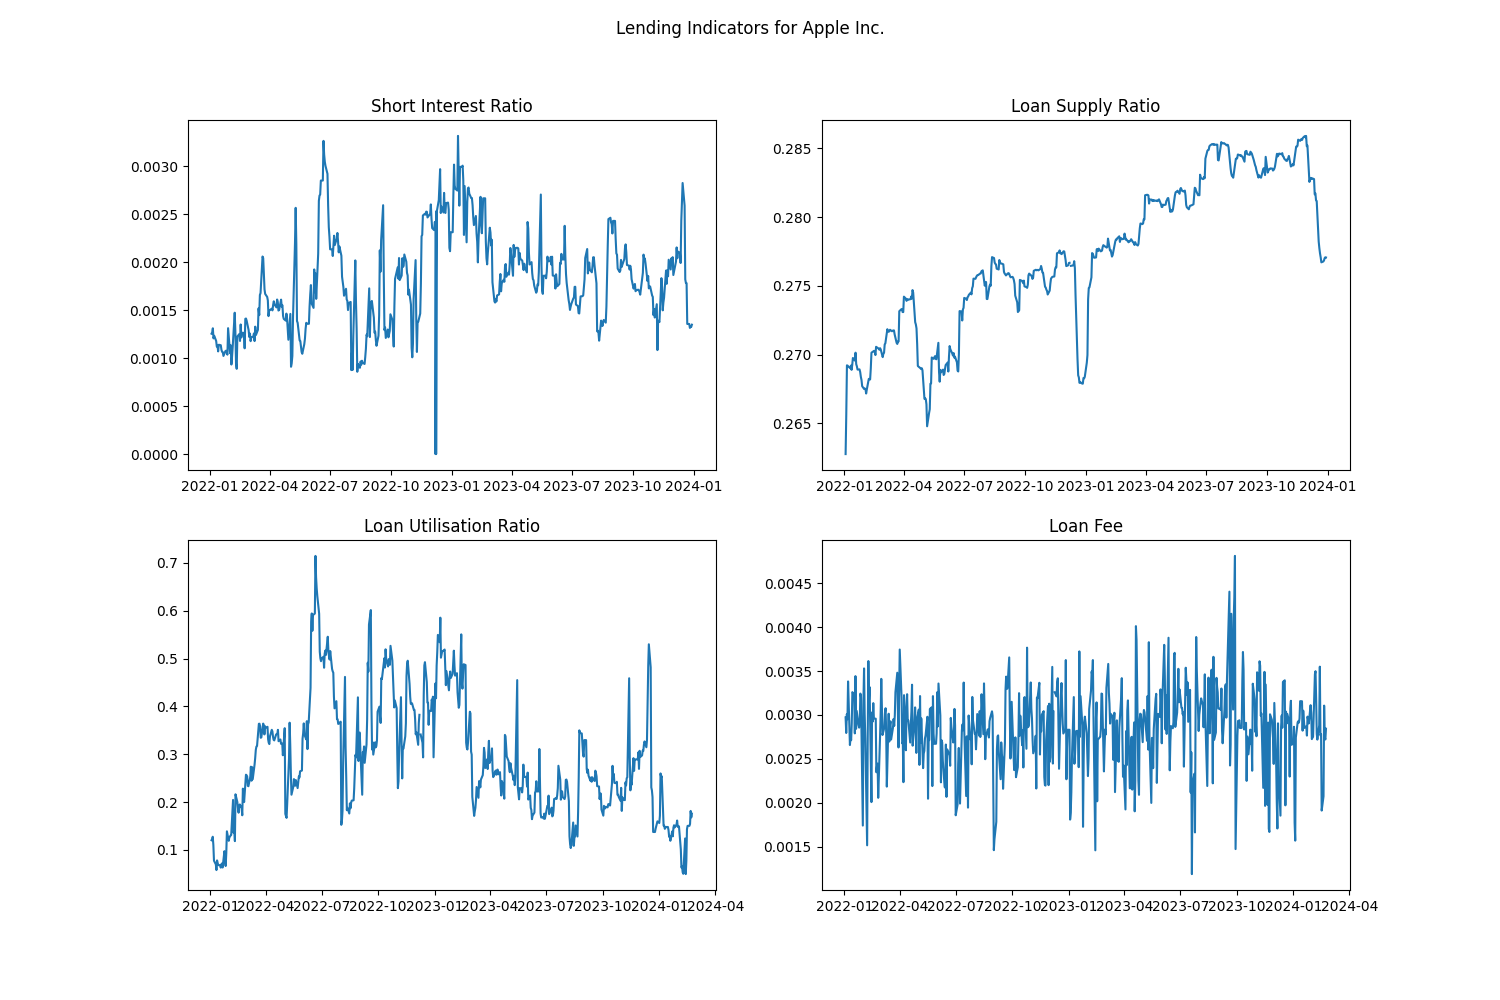
\includegraphics[width=0.75\linewidth]{\PathToOutput/apple_lend_ind.png}
\label{fig:apple_lending_indicators}
\end{figure}

EXPLAIN THE GRAPH


\end{document}